\chapter{Methodology}
\label{chap:Methodology}

Within this chapter, an overview of the tools utilised during the course of the project is provided. 

After a thorough investigation during the early stages of the project, it was decided that the project shall progress as a simulation only model. This was done for a number of reasons:-

\begin{enumerate}
	\item  A simulation based approach negated the possibility of hardware failure, errors or major discrepancies between units. This is especially relevant for this project, where a swarm can be comprised of a large number of units, as the focus can lie with fixing software issues instead of both hardware and software.
	\item A simulation based approach is highly flexible, effective and time efficient. It enables rapid testing of various experimental parameters. 
	\item A simulation based approach is not restricted to available lab space/experimental environments. It is possible to alter the swarm's environment at will, for example if a larger arena or various objects are needed.
	\item A simulation based approach is cost efficient. There are no monetary restraints with regard to adding more robots to the swarm, or costs for repairs on broken robots/replacement parts.
\end{enumerate}
Moreover, as the utilised software package directly simulates real robotic platforms, there will be no need for a major overhaul of the codebase for it to function on a real robot.

\section{Hardware}
\label{section: hardware}

Though the project is conducted entirely in simulation, the agents are based on a real robotic platform, the e-puck (or E-puck, epuck, Epuck). For this reason, an understanding of the capabilities and applications of the platform is essential.

\subsection{E-puck robotic platform}
\label{subsection:hardware-desc}

Developed by \citeauthor{epfl-epuck} at the Autonomous Systems Lab of \'{E}cole Polytechnique F\'{e}d\'{e}rale de Lausanne (EPFL), the e-puck (see Fig \ref{fig:epuck-pic}) is  an open source, two wheeled, differential robot measuring roughly 7cm in diameter. \cite{epfl-epuck}

The e-puck was originally developed to allow students to address a wide range of engineering fields. 

The platform features a wide range of sensing capabilities as standard (see Table \ref{fig:tech-specs}), with the additional option to expand through the use of top and bottom extension slots. (Fig.\ref{fig:flycam}, \ref{fig:randb}) These physical extensions can range from extra sensors, to additional controllers for more computational capabilities (such as an Arduino board).

The flexibility of the platform, coupled with low purchasing costs (owing to the open source nature of the hardware and the software) has thus led to swift adoption by robotics researchers worldwide.
\clearpage

After thorough research of other suitable robotic platforms (see \ref{alt}), the e-puck was chosen as the most desireable base unit to create a swarm. This was due to several factors: -

\begin{enumerate}
	\item The e-puck is flexible. Extensibility allows extra modules to be added if needed.
	\item The e-puck's basic features already have the capabilities required of a swarm agent.
	\item Its relative ease of use and good documentation will enable a quicker development cycle compared to other robots on the market.
\end{enumerate}


\begin{figure}[!b]
	\centering
	\begin{minipage}{.5\textwidth}
		\centering
		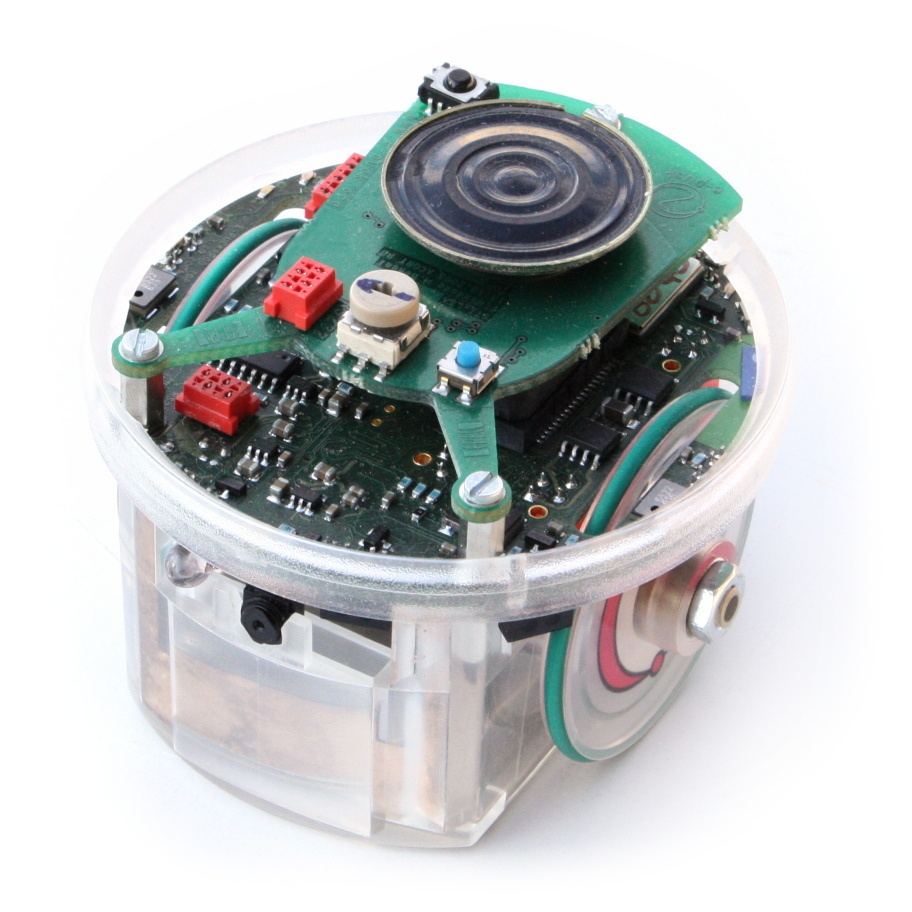
\includegraphics[width=.75\linewidth]{epuck}
		\captionof{figure}{e-puck mobile robot}
		\label{fig:epuck-pic}
	\end{minipage}%
	\begin{minipage}{.5\textwidth}
		\centering
		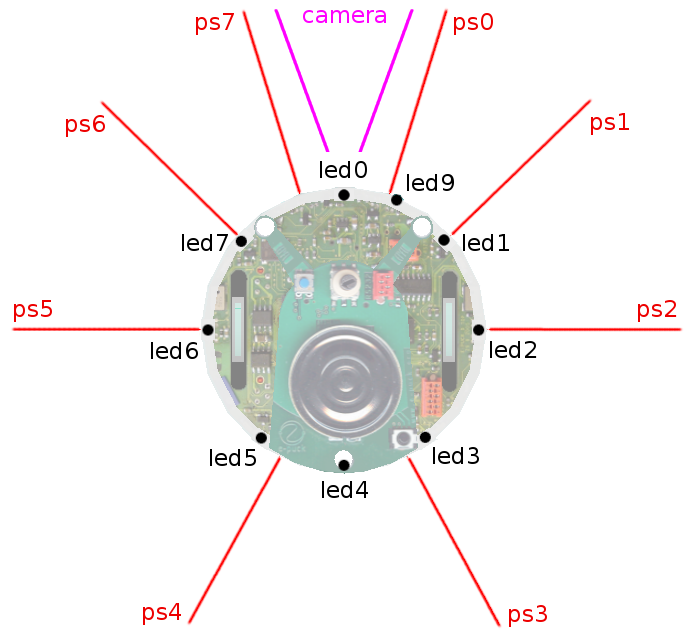
\includegraphics[width=1\linewidth]{e-puck_sensors_and_leds}
		\captionof{figure}{e-puck sensor positions, where ps0 - ps7 denote the positions of the IR sensors}
		\label{fig:epuck-sensors}
	\end{minipage}
\end{figure}

\clearpage


The eight circumferential IR sensors that the robot possesses are crucial in order to exhibit swarm behaviour. These sensors are what allows the robot to "see" its immediate environment and without them the robot will be unable to react to its surroundings.

In addition to this, these sensors allow the use of an IR communication protocol alongside their normal function as proximity or ambient light sensors. In this way, the robots are capable of limited, short range communication with one another.

The e-puck also possesses various wired and wireless communications channels, used primarily to communicate with a host computer. Of note is the Bluetooth radio link, which implements a remote control protocol called the "BTcom protocol". This enables the robot to not only be driven wirelessly, but provides full remote access to the robot's features such as the camera's feed, LED states and sensor data. \cite{epfl-epuck}

Another noteworthy application is the potential use of one robot's body LEDs  signal to other robots its current state. For example, \citeauthor{Christensen:2009:FFS:1650386.1650393} demonstrated a decentralised system of robots that over time will synchronise their flashing with one another. \cite{Christensen:2009:FFS:1650386.1650393}

The e-puck's small size, flexibility and relative low cost are things which would benefit a hardware based research approach.

As can be seen, the array of useful sensors and actuators that are available to the e-puck platform lends itself well to a swarm system application. 

\begin{figure}[!b]
	\centering
	\begin{minipage}{.5\textwidth}
		\centering
	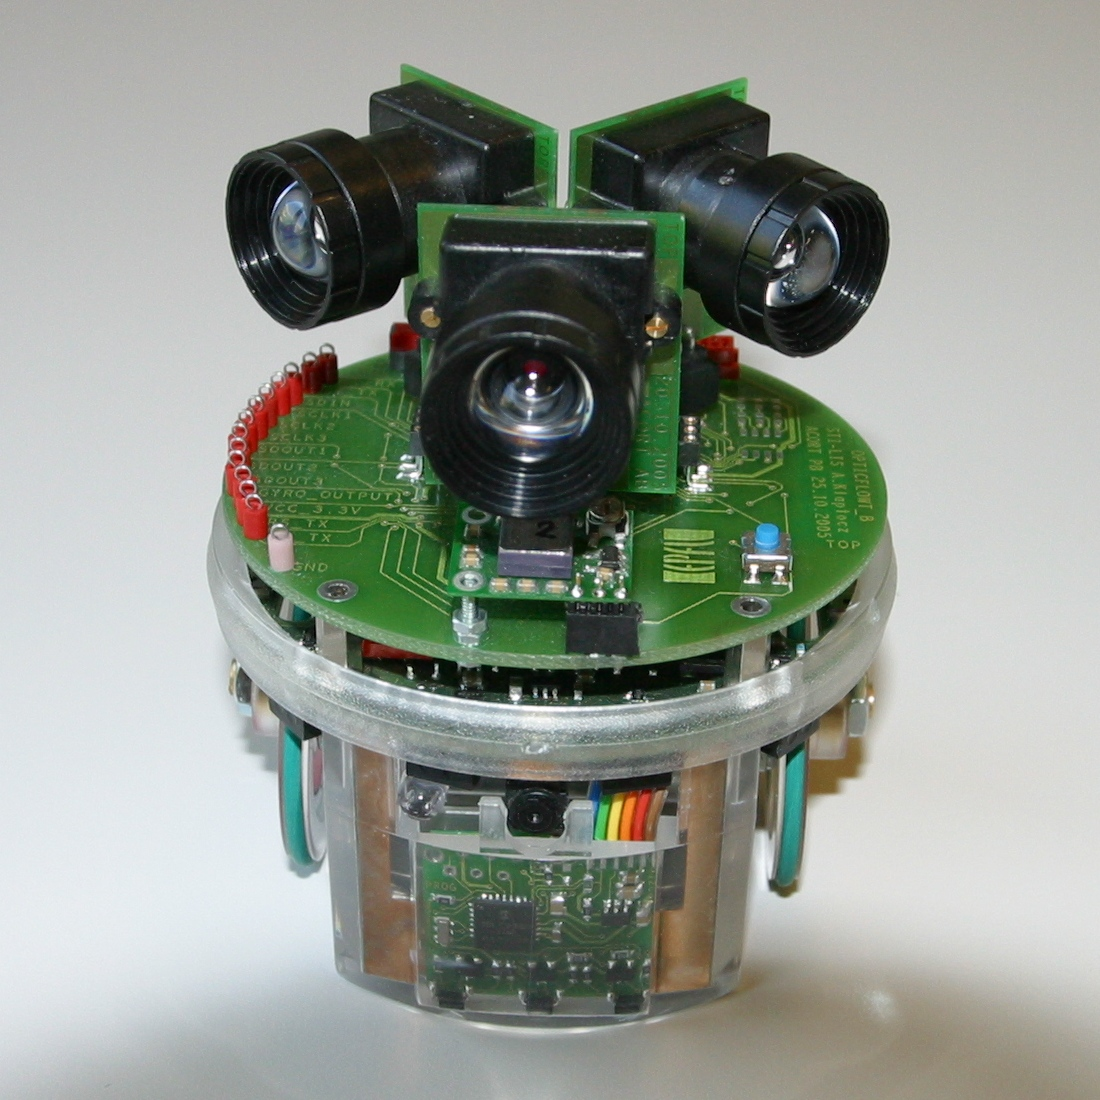
\includegraphics[width=0.7\textwidth]{flycam}
	\caption{\label{fig:flycam}Flycam vision turret.}
	\end{minipage}%
	\begin{minipage}{.5\textwidth}
		\centering
		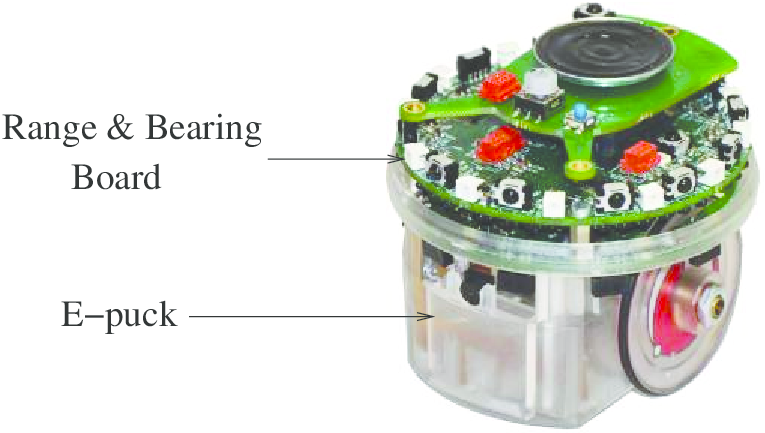
\includegraphics[width=1\linewidth]{randb}
		\captionof{figure}{Range and bearing turret}
		\label{fig:randb}
	\end{minipage}
\end{figure}


\clearpage

\subsection{Alternatives}
\label{alt}

The e-puck platform is not alone in the market of mobile, relatively small robots.

Another potential platform for the project is the Kilobot (Fig. \ref{fig:kilobot}) Developed by Hardvard University's Self-Organizing Systems Research Group and winner of the ``African Robotics Network \$10 Robot Challenge'' \cite{afron}, the Kilobot is a simple and low cost small robot. Envisaged to enable the testing of control algorithms on large swarms accessible to researchers, the Kilobot was designed to prioritise cost and ease of use.  \cite{kilobot} To that end, each unit consists of only \$14 (around \pounds11) worth of parts, requires 5 minutes of assembly time and allows a single operator to control a large group with ease. The control is achieved using an overhead infra-red controller connected to a control station (a computer). This allows a user to broadcast a command or program and have it received by all robots in a swarm within a fixed amount of time, regardless of the number of robots.

Though extremely promising, this platform was not chosen simply for the fact that there was no simulated equivalent available. Also, though cheaper than the vast majority of platforms, the attractive price is only valid if bought or created in bulk.

K-Team's Khepera IV is also an attractive alternative (Fig. \ref{fig:khepera}). The basic feature set of the Khepera IV far outstrips that of the e-puck, with the former housing a WiFi chipset, 4 IR ground sensors as standard, 5 sonar sensors, a run time of 5 hours and an extension ecosystem. In addition to this, the robot embeds a complete Linux operating system, allowing "almost any existing library" to be easily ported. \cite{khepera}

This was not chosen as though it is technically superior, the extra functionality does not offer any substantial gains over the e-puck for this application. It is not open source, so not as widespread as the e-puck. In addition to this, the Khepera IV is significantly more expensive than the e-puck, at 2650 CHF (around \pounds2140) for a single unit.

Bot'n Roll's ONE A unit was also considered. Aimed more toward beginners rather than researchers, the ONE A is a differential wheeled robot with an LCD screen mounted on an Arduino programmable board. It comes with two forward facing IR sensors used for distance sensing. \cite{onea} This was not chosen as though it provided a few external connections for additional sensors, the extra sensors did not come as standard and has to be soldered manually. At 199 EUR, it also provided very little value for money compared with other platforms, and its simplicity is liable to be a hinderance.
\begin{figure}[h]
	\centering
	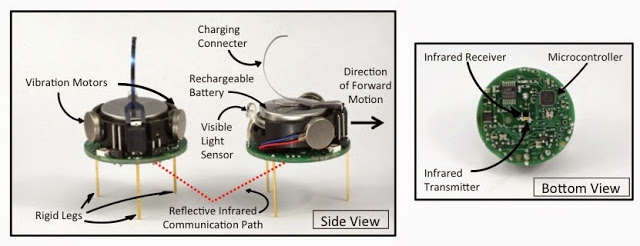
\includegraphics[width=1\textwidth]{kilobots}
	\caption{\label{fig:kilobot}Kilobot}
\end{figure}

\begin{figure}[h]
	\centering
	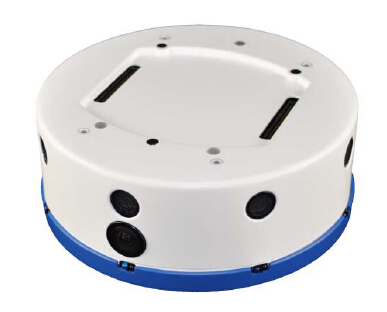
\includegraphics[width=0.5\textwidth]{khepera}
	\caption{\label{fig:khepera}Khepera IV}
\end{figure}
\clearpage

\section{Software}

As the project is an entirely simulation based study, the utilised software tools are of paramount importance. 

\subsection{Webots simulator}
\label{webots}

Webots, developed by Cyberbotics, is a professional development and simulation environment for mobile robots. Cyberbotics is at the forefront of robot simulation, with Webots being used by over 1284 universities and research centres worldwide. \cite{cyberbotics-about}

\begin{figure}[h]
	\begin{minipage}{.75\textwidth}
		\centering
		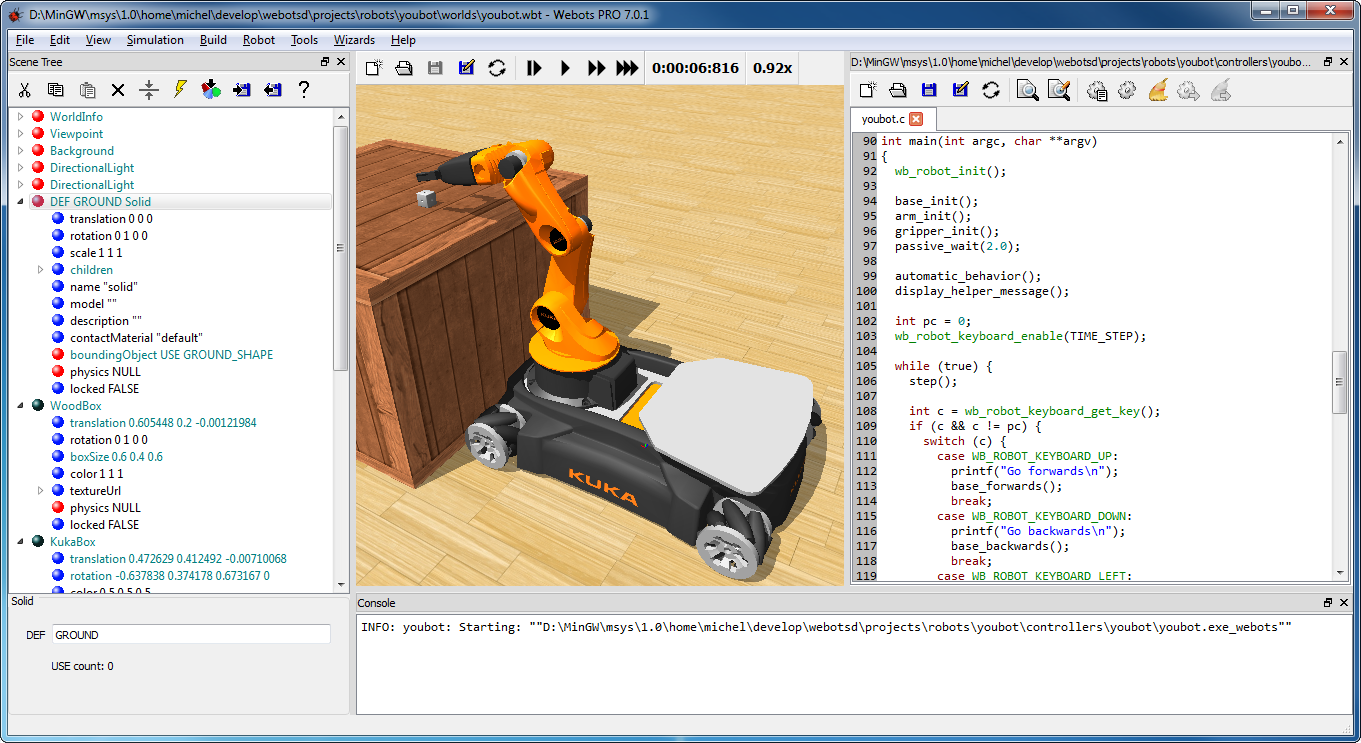
\includegraphics[width=1.35\linewidth]{webots-screen}
		\captionof{figure}{Webots simulator}
		\label{fig:screen}
	\end{minipage}
\end{figure}

Webots was chosen as the desired development environment as it allows quick creation of complex robotics setups, as well a streamlined way to set up a virtual operating environment. It features a built in integrated development environment for programming, should a user wish to use this. In addition to this, the simulator utilises the Open Dynamics Engine (ODE) in order to simulate rigid body dynamics and collision detection. This allows realistic physics to be accurately simulated in a virtual environment.

The simulator also allows cross compilation of code onto live robots, cutting down development time if the user wishes to test on a live platform.

Another advantage afforded by Webots is that the distribution comes pre-packaged with a host of modifiable robot models, aimed at closely simulating any real life counterparts. Where this project is concerned, there already exists a virtual e-puck model. This e-puck is, for all intents and purposes, as functional as the hardware equivalent, and possesses all of the same sensors and actuators.

Conducting experiments in Webots is also streamlined. It features the ability to advance through a simulation step-by-step, at a time step defined by the user. This is useful for close analysis of robot behaviour. The virtual camera can be oriented in three dimensions and enables the taking of pictures and videos, also useful for experimental analysis and documentation.

There exists C, C++, MATLAB, Java and Python libraries for the functions of robot controller programs and Cyberbotics' documentation of this API aids in speeding up the development cycle.

\subsubsection{Concepts}

To fully understand Webots, some basic underlying principles have to be outlined. A simulation is defined as a \textit{world}, containing \textit{models} (which includes static objects and robots), and \textit{controllers} are executed on these models if they are able to.

Each \textit{world} is defined by a .wbt file, which contains all of the information about that simulation. Within this file, everything from the number and type of robots to the amount of ambient light present are defined.

A robot \textit{model} is defined by a .proto file, which contains information regarding that type of robot. For example, this file could contain the positions of and number of sensors a particular robot has.

A robot \textit{controller} is the program that executes on the robot itself. This is where the behaviour of the robot is defined and is written in a programming language chosen from those Webots supports. In the case of this project, C++ was chosen.

\subsection{C++ programming language}

Released as a commercial product in 1985, C++ was developed by Danish computer scientist Bjarne Stroustrup. Stroustrup developed the language with the aim of integrating object-oriented programming into the C language. This was viewed as an improvement to the C language, making the language easier to use for larger software development projects without sacrificing the low-level memory management, speed and portability that C is renowned for. \cite{c++-history}

C++ is in use in many different industries and has a very widespread adoption. It is currently positioned in third place on the TIOBE Programming Community index, which is a measure of the popularity of programming languages worldwide. \cite{tiobe}

It was decided that C++ was to be used for this project for the following reasons:-

\begin{enumerate}
	\item The language is fast. C++ performs calculations relatively quickly in comparison with other languages.
	\item C++ allows a high degree of user code optimisation, which could improve performance especially in resource limited applications.
	\item C++ is object-oriented. This aids in the software design process by enabling a higher level of abstraction.
	\item C++ is well documented. With over 30 years of history and frequent revisions, most errors and issues have been encountered and solved in the past.
	\item It is suitable for embedded and robotics applications. It is currently in widespread use within the robotics industry, with C++ being one of the main supported languages of the ROS (Robot Operating System) framework.
\end{enumerate}